\subsection{Experiment 2: Context-Guided Relationship Selection}
\label{sec:exp2}

Experiment~2 asks which of two displayed relationships a model applies to a new
target. Reference cities instantiate strong and weak response regimes, a cue assigns City
C to one, and City C observations accumulate from $k=0$ to $k=4$. Paired prompts
share their numeric content; the correct- and wrong-context arms change only the
cue. Because the semantic descriptions state which regime is stronger, the novel
induction test uses arbitrary labels whose mapping changes by episode
(Appendix~\ref{app:coin-city}).

\begin{figure}[!ht]
\centering
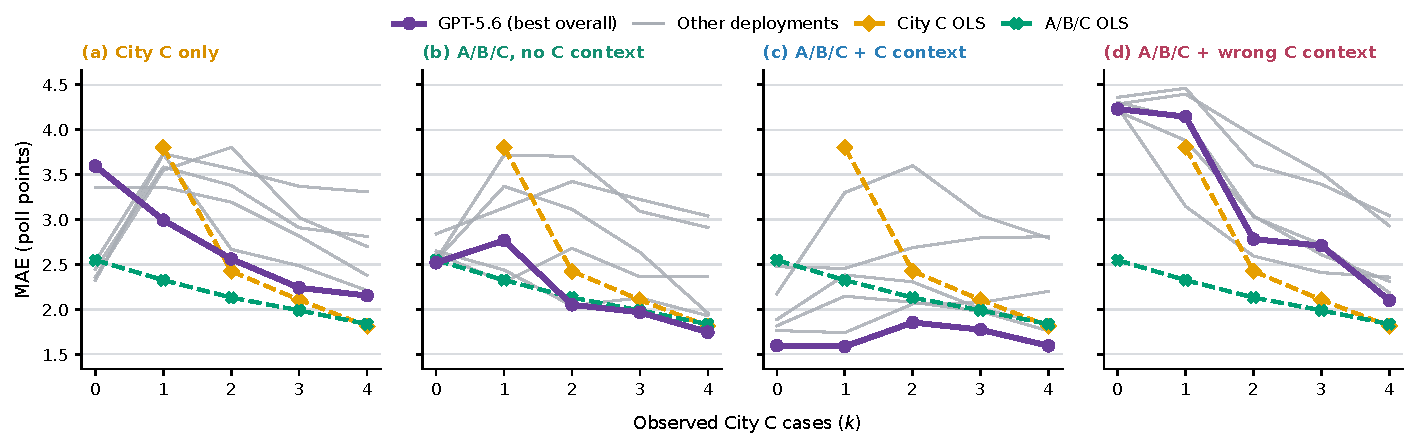
\includegraphics[width=\linewidth]{figures/exp2_coin_city_results.pdf}
\vspace{3pt}
\begin{minipage}{\linewidth}
\centering
\footnotesize
\setlength{\tabcolsep}{4pt}
\resizebox{\linewidth}{!}{%
\begin{tabular}{l r rrrr rr}
\toprule
& & \multicolumn{4}{c}{Forecast MAE [95\% CI]} & \multicolumn{2}{c}{$\rho(\hat g,g_C)$} \\
\cmidrule(lr){3-6}\cmidrule(lr){7-8}
Model & Paired $n$ & Target only & No C context & $+$ C context &
$+$ wrong C context & No context & $+$ context \\
\midrule
\micon{claude.png}~Opus~4.8 & 250 & 2.32 [2.20,\,2.46] & 2.65 [2.41,\,2.89] & \textbf{1.82} [1.64,\,2.02] & 4.20 [3.87,\,4.54] & $-.06$ & \textbf{.70} \\
\micon{claude.png}~Opus~5 & 250 & 2.36 [2.12,\,2.59] & 2.62 [2.38,\,2.84] & \textbf{1.76} [1.57,\,1.99] & 4.25 [3.92,\,4.57] & $-.01$ & \textbf{.62} \\
\micon{openai.png}~GPT-5.6 & 250 & 3.60 [3.28,\,3.94] & 2.52 [2.33,\,2.75] & \textbf{1.60} [1.42,\,1.77] & 4.23 [3.90,\,4.55] & $-.04$ & \textbf{.68} \\
\micon{deepseek.png}~V4-Pro & 250 & \textbf{2.45} [2.27,\,2.61] & 2.84 [2.55,\,3.15] & 2.47 [2.19,\,2.77] & 4.36 [4.01,\,4.74] & $-.03$ & \textbf{.52} \\
\micon{kimi.png}~K3 & 250 & 3.35 [3.04,\,3.67] & 2.55 [2.32,\,2.78] & \textbf{1.89} [1.66,\,2.13] & 4.31 [3.98,\,4.62] & $-.02$ & \textbf{.59} \\
\micon{gemini.png}~3.6 Flash & 250 & 2.53 [2.35,\,2.73] & 2.55 [2.31,\,2.80] & \textbf{2.17} [1.89,\,2.48] & 4.29 [3.94,\,4.66] & $.08$ & \textbf{.56} \\
\bottomrule
\end{tabular}
}
\end{minipage}
\caption{\textbf{Context improves zero-shot forecasts and regime assignment across
six deployments.} Panels add references, the correct cue, then an inverted cue
as City C observations accumulate. Gray lines are deployments, purple the best
overall, and dashed lines OLS references. The table reports $k=0$ MAE and slope
correlation with 95\% intervals (Appendix~\ref{app:coin-city-results}).}
\label{fig:coin-city-results}
\end{figure}

\begin{wrapfigure}{r}{0.35\textwidth}
\vspace{-1.0em}
\centering
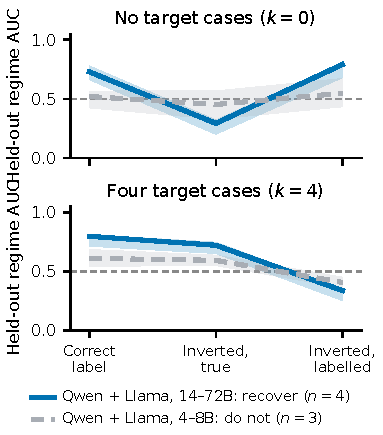
\includegraphics[width=\linewidth]{figures/exp2_symbol_decoding.pdf}
\vspace{-0.8em}
\caption{\textbf{The decoded regime follows the arbitrary cue, then the truth once
evidence arrives.} Held-out regime AUC, 88 sealed episodes. Open markers do not
reject their permutation null; gray marks checkpoints whose forecasts do not
recover the mapping.}
\label{fig:coin-city-symbol-decoding}
\vspace{-1.0em}
\end{wrapfigure}
\textbf{Selection and revision.} The cue lowers zero-shot error for every
deployment, by $0.37$ to $0.92$ poll points with all six paired intervals
excluding zero, and at $k=0$ every deployment matches or beats a context-blind
OLS benchmark (Appendix Table~\ref{tab:coin-city-vs-ols}). An inverted cue
reverses the assignment. By $k=4$, however, its advantage narrows to
$0.12$--$0.23$ points as target evidence takes over. Performance approaches reference policies derived from the prompt: the best no-cue
result is within $2\%$ of its $2.28$-point floor, while a reader that estimates the
named regime from four noisy reference rows obtains $1.78$ MAE. Deployments reach
$1.60$--$2.47$, and can improve on that plug-in reference by shrinking toward the
known regime mean (Appendix~\ref{app:coin-city-probe-ceilings}).

\textbf{The cue selects a displayed reference, not a prior on its words.}
Partialling out the regime distinguishes these accounts: at $k=0$, neither
reference loads when its cases are absent, both load equally without a cue, the
correct cue loads the named reference ($.51$--$.86$) but not the other
($.04$--$.10$), and inversion moves loading to the cue-named but incorrect reference
($.61$--$.90$). Inherited source noise also caps implied-slope correlations near
$.66$, rather than $.996$ (Appendix~\ref{app:coin-city-reference-selection}).

\textbf{Induction of a novel mapping.} On the original population, twelve of fifteen
systems recover it at $k=0$, including all five hosted systems. A harder
population compresses scores toward chance without reordering checkpoints, moving
the threshold at which recovery is detectable; parameter count alone still does
not explain the transition across families
(Appendix~\ref{app:coin-city-robustness}). Semantic probes reach AUC $1.000$, but
input embeddings alone already reach $1.000$; under arbitrary labels that control
falls to $.555$, and the decoded regime follows the label at $k=0$ and the truth
at $k=4$ (Figure~\ref{fig:coin-city-symbol-decoding}). Decoding and forecasts agree for all seven
probed checkpoints on this population. The harder population compresses the four Qwen3
symbol-arm scores toward chance while preserving their order, so which checkpoints
clear significance moves even though none reverse; the agreement bounds what the
probe reads on these episodes rather than locating a scale threshold. Patching
those states shifts Qwen3-14B's forecast by $.333$ at $k=0$ ($p<.0001$) but not at
$k=4$, showing that the induced label representation contributes causally to this
checkpoint's zero-shot forecast
(Appendix~\ref{app:coin-city-mechanistic-probe}).


Together, the paired interventions show a displayed relationship being selected,
reversed, and then overridden by target evidence. The deterministic
pick-a-reference-then-fit policy is the hypothesis here rather than a rival: it
matches or beats most deployments at $k=0$, and the contribution is evidence that
deployments implement it---inverting the cue inverts the forecast, the implied
slope carries the named reference's own sampling error, and the selected regime is
decodable and causally necessary. City C displays no rows at $k=0$, so this is not
in-context fitting on the target.
The cue is binary and the regimes well separated; within-regime variation is too
small to test exact coefficient recovery; and causal patching covers one of seven
open checkpoints, with hosted deployments tested only behaviorally.
